%!TEX root=main.tex

\section{Performance Tests} \label{performance}

Performance testing is a critical part of development, so it is important to demonstrate Pasithea's performance under different loads and its ability to log many -- potentially thousands -- of incoming requests in a short amount of time. 
In other words, it must respond fast enough to keep malicious users interested while also being stable enough to receive high volumes of incoming requests. 
To test this, we ran a series of benchmarks using the Apache Bench (ab) tool~\cite{ab}. 
This tool allows us to designate a number of completed requests to be sent to our API honeypot while varying the number of simulated concurrent users. 
The results from these tests are displayed in Fig.~\ref{fig:R/s} and Fig.~\ref{fig:T/R}. 

\begin{figure}[b]
   \centering
   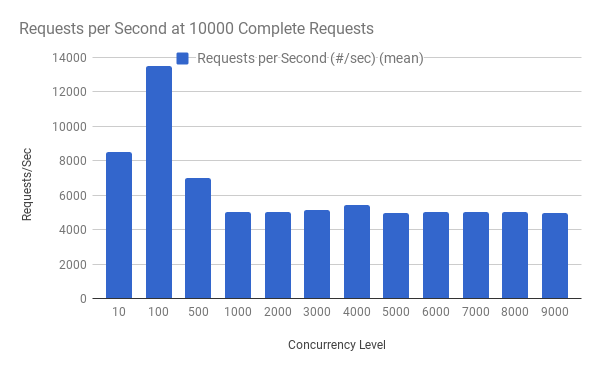
\includegraphics[width=2.5in]{images/RequestsperSecond.png} 
   \caption{Requests processed per second at varying concurrency levels}
   \label{fig:R/s}
\end{figure}

We researched a baseline response time for a RESTful API to give this data appropriate context. 
In doing so, we discovered two separate internal tests from software development and web monitoring companies, 3PillarGlobal~\cite{3Pillar} and Site24x7~\cite{site24x7}. 
Paired with some research on the human perception of performance~\cite{performance}, we concluded that a 300-ms response time is expected under normal traffic conditions in order for the API honeypot to appear realistic. 
Data collected on Pasithea indicates that we fall well within this range given a concurrency level of 500 simultaneous users. 
In addition, we continued tests at much higher concurrency levels to assess how well Pasithea would perform under extreme stress, like the attempts we saw on the G-star API. 
Pasithea can, with time, handle a concurrency level of over 9000 simultaneous requests while still logging more than 90\% of the requests received.

\begin{figure}[t]
   \centering
   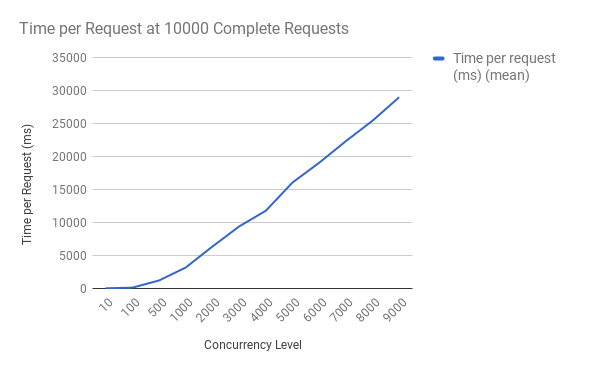
\includegraphics[width=2.5in]{images/TimeperRequest.png} 
   \caption{Mean time to complete a single request at varying concurrency levels}
   \label{fig:T/R}
\end{figure}

Since our implementation of request/response for Pasithea was deliberately kept very simple (only responding with 404 errors), we have thus far been unsuccessful in driving Pasithea hard enough during performance testing to reach a point where it is unable to handle a significant amount of requests.  
Pasithea hits a $R/s$ plateau at a concurrency level of 1000, see Fig.~\ref{fig:R/s} but continues to perform well at 9000.
With enough storage space, we believe that Pasithea could withstand a substantial attack, such as the one seen on G-star, and be able to log information about the attack for analysis.
